\chapter{\uppercase{Results and Performance Analysis}}
\label{chap5}

This chapter evaluates three complementary AgentOS subsystems: the context-paging engine, the model-backed planner, and the global agent scheduler. The context experiments measure evidence visibility, retrieval quality, and active-context reduction. The planner experiment measures selection of the registered AgentOS tools. The scheduler experiments measure execution reliability and the latency trade-off introduced by priority aging. These evaluations are reported as project-specific measurements rather than as claims on an official external leaderboard.

\section{\uppercase{Evaluation protocol}}

The evaluation used the AgentOS function catalogue generated from the registered agent registry. Each registered agent was exposed as an OpenAI-compatible function with a task argument and an optional context argument. The model endpoint was Groq using \texttt{openai/gpt-oss-120b}. The same catalogue and system prompt were used for every trial. Because every task in this dataset required at least one registered agent, the request used required tool-call mode. A 25-second inter-request delay was applied to avoid token-per-minute throttling.

The experiments use deterministic local smoke sets, controlled synthetic scheduler workloads, and a fixed pilot subset of the LoCoMo long-term conversational-memory benchmark. Each comparison keeps the task or question set, configuration, and scoring definitions fixed across systems. The results are intended as implementation and reliability evidence rather than as statistically representative estimates of general model or production-system performance.

\section{\uppercase{Context-paging engine}}

The context-paging engine was evaluated using two complementary datasets. The first was a deterministic synthetic smoke set designed to verify paging, telemetry, retrieval, and active-context reduction. The second was a pilot derived from annotated LoCoMo questions. The configurations compared complete-context access, recent-message truncation, direct vector retrieval, and AgentOS paging, which combines a larger semantic candidate pool with one-message neighbourhood expansion and lexical reranking. A successful retrieval trial means that the annotated evidence required to answer the question was visible in the active context or returned by paging; it is not an end-to-end language-model answer score.

\subsection{Synthetic smoke evaluation}

The synthetic run expanded five seed scenarios into 50 deterministic conversational questions and executed 400 configuration trials. AgentOS paging was evaluated at similarity thresholds of 0.40, 0.45, 0.50, 0.55, and 0.60. Table~\ref{tab:context-synthetic-results} reports the authoritative aggregate values. The full-context configuration is a quality-control reference and does not perform retrieval.

\begin{table}[H]
\centering
\scriptsize
\caption{Synthetic context-paging evaluation}
\label{tab:context-synthetic-results}
\begin{tabular}{>{\raggedright\arraybackslash}p{4.2cm}rrrr}
\toprule
Configuration & Success (\%) & Recall@5 (\%) & Token reduction (\%) & Page-in time (ms) \\
\midrule
Full-context control & 100.0 & N/A & 0.0 & N/A \\
Recent-message truncation & 20.0 & N/A & 55.6 & N/A \\
Vector RAG & 100.0 & 100.0 & 0.6 & 365 \\
AgentOS paging ($\tau=0.40$) & 90.0 & 87.5 & 35.3 & 364 \\
AgentOS paging ($\tau=0.45$) & 82.0 & 77.5 & 42.1 & 371 \\
AgentOS paging ($\tau=0.50$) & 82.0 & 77.5 & 43.6 & 352 \\
AgentOS paging ($\tau=0.55$) & 78.0 & 72.5 & 45.8 & 382 \\
AgentOS paging ($\tau=0.60$) & 70.0 & 62.5 & 48.7 & 362 \\
\bottomrule
\end{tabular}
\end{table}

The synthetic results confirm that paging is operational and expose the trade-off introduced by the similarity threshold. Vector RAG achieved 100\% success and 100\% Recall@5 on this deliberately simple dataset, but reduced active-context tokens by only 0.6\%. AgentOS paging at $\tau=0.40$ achieved 90\% success, 87.5\% Recall@5, and 35.3\% token reduction. Increasing the threshold improved token reduction to 48.7\% at $\tau=0.60$, but reduced success to 70\% and Recall@5 to 62.5\%. Page-in latency ranged from 352 to 382 ms across the tested configurations, while repeated embedding work was reduced by the embedding cache to approximately 0.001 ms. Recent-message truncation reduced the active context by 55.6\% but achieved only 20\% success, demonstrating that retaining only the newest messages is insufficient when the required evidence is older than the active window.

\subsection{LoCoMo pilot evaluation}

The LoCoMo pilot used a fixed subset of annotated long-term conversational questions and executed 800 configuration trials. The AgentOS operating point is reported for the best observed threshold region ($\tau=0.20$--$0.30$); this is a pilot observation rather than a threshold selected from a held-out development set.

\begin{table}[H]
\centering
\scriptsize
\caption{LoCoMo pilot context-retrieval evaluation}
\label{tab:context-locomo-results}
\begin{tabular}{>{\raggedright\arraybackslash}p{4.5cm}rrrr}
\toprule
Configuration & Success (\%) & Recall@5 (\%) & MRR@5 (\%) & Token reduction (\%) \\
\midrule
Full-context control & 100.0 & -- & -- & 0.0 \\
Recent truncation & 6.0 & -- & -- & 95.0 \\
Vector RAG & 22.0 & 18.2 & 7.1 & 93.1 \\
AgentOS paging ($\tau=0.20$--$0.30$) & 35.0 & 32.8 & 13.7 & 92.9 \\
\bottomrule
\end{tabular}
\end{table}

On the more difficult conversational data, AgentOS paging improves retrieval success by 13 percentage points over vector RAG and improves Recall@5 by 14.6 percentage points, while maintaining approximately the same 93\% reduction in active-context tokens. This indicates that neighbourhood-aware paging is better suited to multi-turn evidence than retrieving isolated messages alone. The absolute scores also show that long-term memory retrieval remains an open problem; these results should not be described as perfect question answering.

\section{\uppercase{Planner and tool selection}}

Exact tool-set accuracy is the fraction of trials for which the selected agent functions exactly matched the expected set. Required-tool recall is the fraction of trials in which every expected function was selected. The end-to-end measures count a failed model tool call as an incorrect outcome. Provider errors and model tool-call failures are recorded separately so that infrastructure problems are not confused with routing errors.

\section{\uppercase{Results}}

Table~\ref{tab:planner-tool-results} summarises the 50-trial run. Thirty-eight trials produced the expected tool set, while twelve trials failed at the tool-call stage. No provider errors were recorded. The aggregate latency, computed from the category-level means weighted by their trial counts, was 1003.36 ms.

\begin{table}[H]
\centering
\caption{AgentOS tool-selection adapter results}
\label{tab:planner-tool-results}
\begin{tabular}{>{\raggedright\arraybackslash}p{7.2cm}r}
\toprule
Measure & Result \\
\midrule
Total trials & 50 \\
Successful API trials & 50 \\
Correct tool sets & 38/50 (76.0\%) \\
End-to-end exact tool-set accuracy & 38/50 (76.0\%) \\
End-to-end required-tool recall & 38/50 (76.0\%) \\
Model tool-call failures & 12 (24.0\%) \\
Provider or transport errors & 0 \\
Weighted mean latency & 1003.36 ms \\
\bottomrule
\end{tabular}
\end{table}

\begin{figure}[H]
\centering
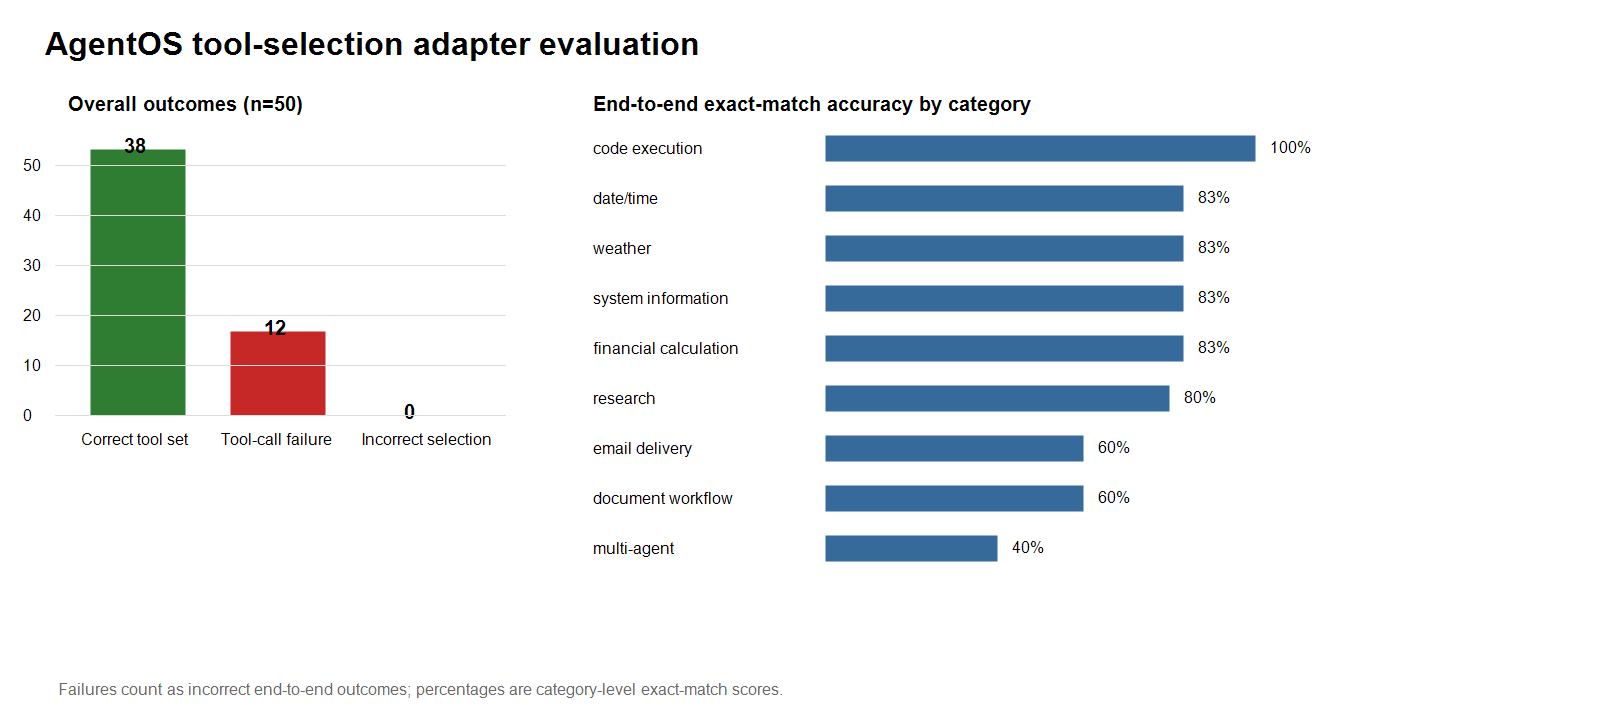
\includegraphics[width=0.98\textwidth]{5/figures/planner_tool_selection_results.png}
\caption{Overall outcomes and per-category end-to-end accuracy for the AgentOS tool-selection adapter.}
\label{fig:planner-tool-selection-results}
\end{figure}

The category results indicate strong performance in code execution, with 100\% exact-match accuracy, followed by date and time, weather, system information, and financial calculation at 83.3\% each. Research achieved 80.0\%. Email delivery and document workflow achieved 60.0\% each, while multi-agent coordination was the weakest category at 40.0\%. The same categories also exhibited comparatively high latency, with multi-agent coordination averaging 1338 ms and research and document workflow averaging 1287 ms and 1272 ms, respectively. These results suggest that the principal limitation is tool-call compliance and routing complexity rather than provider availability. The required-call setting made these failures explicit instead of allowing a prose response to be counted as a successful request.

\section{\uppercase{Agent scheduler}}
\label{sec:agent-scheduler-evaluation}

The scheduler evaluation consisted of a deterministic smoke suite and a controlled workload benchmark. The smoke suite executed 21 trials covering concurrency and task limits, cooperative preemption, cumulative token budgets, oversized jobs, priority ordering, quota retry, and runner failure; all 21 completed successfully. The workload benchmark compared the implemented priority-aging policy with an admission-aware FIFO policy using the same seeded workloads, service-time distributions, and priority values. Each policy and workload profile was repeated ten times, producing 40 trials in total. Persistence was stubbed, so the measurements capture in-process scheduling and asynchronous runner behaviour rather than Redis or MongoDB network overhead.

\begin{table}[H]
\centering
\scriptsize
\caption{Priority-aging scheduler versus FIFO}
\label{tab:chapter-scheduler-results}
\begin{tabular}{>{\raggedright\arraybackslash}p{3.0cm}>{\raggedright\arraybackslash}p{2.3cm}rrrr}
\toprule
Workload & Policy & Throughput (jobs/s) & Queue $P_{95}$ (ms) & High-priority queue $P_{95}$ (ms) & End-to-end $P_{95}$ (ms) \\
\midrule
Steady state & Priority aging & 254.27 & 218.06 & 65.18 & 233.44 \\
Steady state & FIFO & 258.00 & 214.48 & 206.00 & 229.96 \\
Queue contention & Priority aging & 85.92 & 511.92 & 101.41 & 537.25 \\
Queue contention & FIFO & 85.84 & 508.35 & 459.55 & 536.64 \\
\bottomrule
\end{tabular}
\end{table}

\begin{figure}[H]
\centering
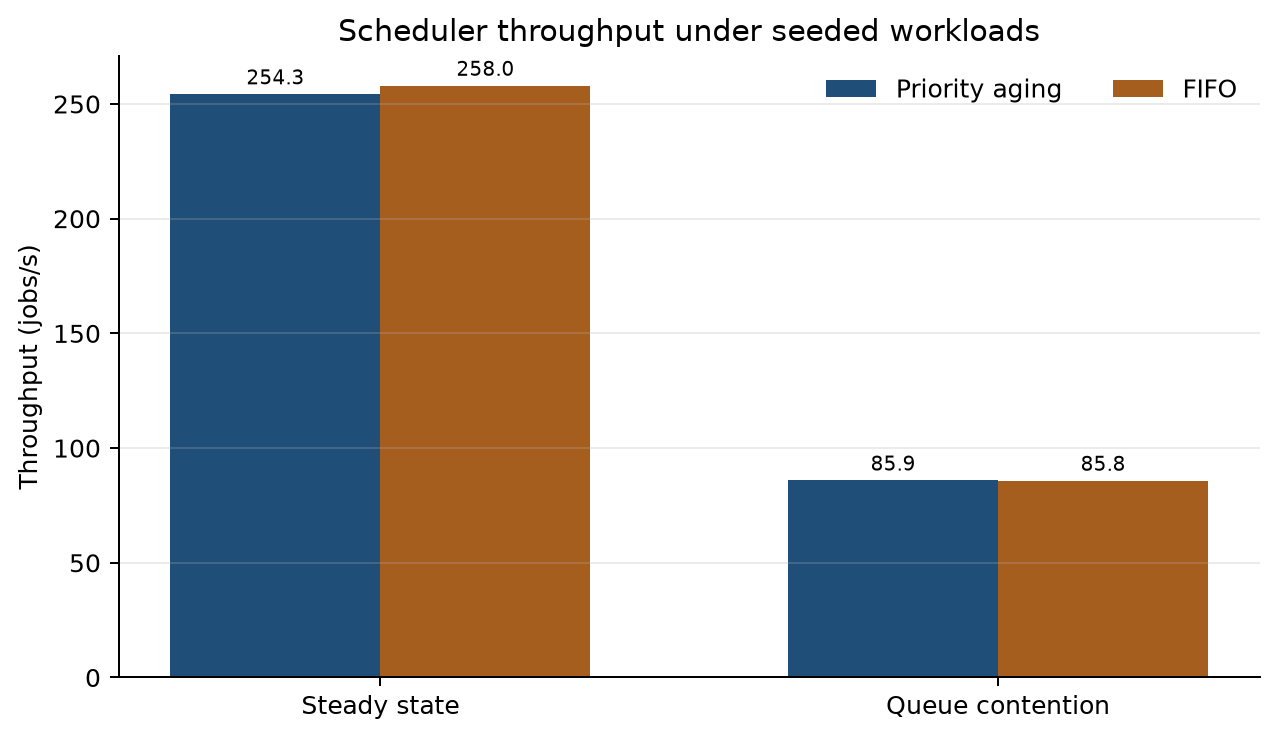
\includegraphics[width=0.86\textwidth]{5/figures/scheduler_throughput_baseline.png}
\caption{Measured scheduler throughput under steady-state and queue-contention workloads}
\label{fig:chapter-scheduler-throughput}
\end{figure}

\begin{figure}[H]
\centering
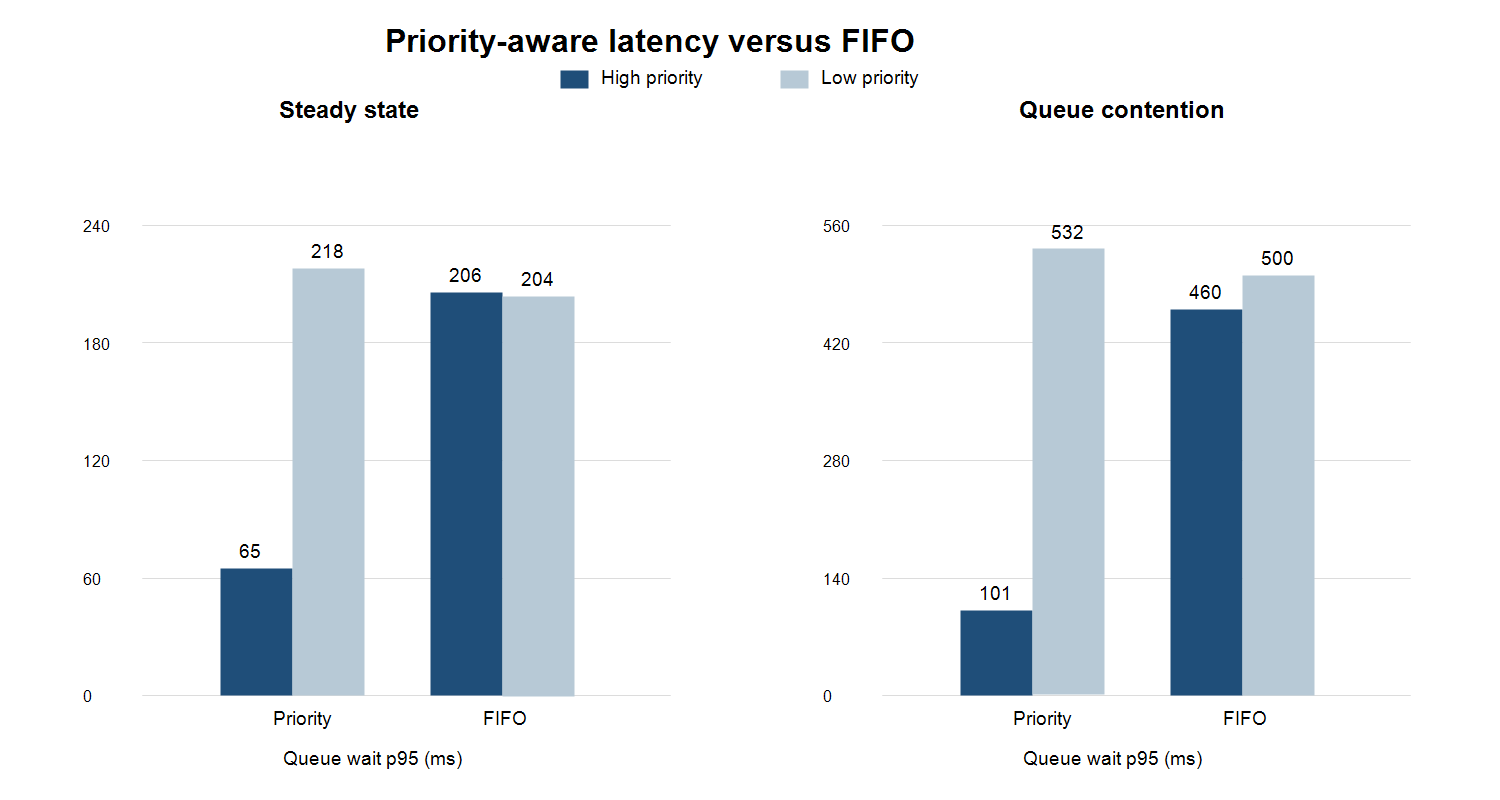
\includegraphics[width=0.88\textwidth]{5/figures/scheduler_priority_latency.png}
\caption{High- and low-priority queue-wait $P_{95}$ under priority aging and FIFO; the legend is positioned above the plotting area for clarity}
\label{fig:chapter-scheduler-latency}
\end{figure}

Priority aging reduced high-priority queue-wait $P_{95}$ by 140.82 ms in steady state and by 358.14 ms under contention, corresponding to approximate reductions of 68\% and 78\% relative to FIFO. Throughput remained effectively unchanged under contention (+0.10\%) and decreased by 1.45\% in steady state. Overall queue-wait $P_{95}$ increased by approximately 3.6 ms in both profiles because the policy protects urgent work by allowing lower-priority jobs to wait longer. No concurrency-limit violations or cross-task completion imbalance were observed. These measurements should be interpreted as a controlled same-host comparison, not as a production-capacity claim.

\section{\uppercase{Interpretation and limitations}}

The 76.0\% end-to-end result should be interpreted as a preliminary AgentOS routing measurement. It is not an official BFCL score, because the evaluation uses the AgentOS registry, a project-specific task set, and AgentOS-specific expected tool mappings. The aggregate score includes all 50 trials and therefore incorporates the 12 tool-call failures. The more informative system-level result is consequently 38 correct outcomes out of 50 total trials, together with a 24.0\% tool-call failure rate and zero provider errors.

The next evaluation increment should expand the planner task set with paraphrased email, document, research, financial, and multi-agent cases, and compare required-call mode with automatic tool-choice mode. The context engine should be evaluated on a larger held-out LoCoMo or LongMemEval sample with a fixed development/test threshold split and an answer-quality judge. The scheduler should be replayed using anonymised production-like arrival traces, non-stubbed persistence, and provider latency. Across all three tracks, future reporting should include confidence intervals, raw trial identifiers, and a clear separation between smoke-test conformance and externally generalisable performance.
